\begin{table}[h]
    \centering
    {\scriptsize
    \caption{Number of floating-point operations for different dimension sizes for $a,b,c,d,e,f$. For the other three contractions abcd,adef$\rightarrow$dbef, aabcd,adeef$\rightarrow$bcf and abcd,adef$\rightarrow$cbef, the sizes of the tensors are changed in an analogous manner.}
    \label{tab:dimensions}
    \begin{tabular}{ccc}  
        \toprule
        \textbf{Dimension Size} & \textbf{aabcd,adeef}$\rightarrow$\textbf{dcf} & \textbf{FLOPs} \\
        \midrule
        2  & A:(2,2,2,2,2), B:(2,2,2,2,2) & 2.11  \\
        5  & A:(5,5,5,5,5), B:(5,5,5,5,5) & 4.49  \\
        10 & A:(10,10,10,10,10), B:(10,10,10,10,10) & 6.30  \\
        15 & A:(15,15,15,15,15), B:(15,15,15,15,15) & 7.36  \\
        20 & A:(20,20,20,20,20), B:(20,20,20,20,20) & 8.11  \\
        25 & A:(25,25,25,25,25), B:(25,25,25,25,25) & 8.69  \\
        30 & A:(30,30,30,30,30), B:(30,30,30,30,30) & 9.16  \\
        35 & A:(35,35,35,35,35), B:(35,35,35,35,35) & 9.56  \\
        40 & A:(40,40,40,40,40), B:(40,40,40,40,40) & 9.91  \\
        45 & A:(45,45,45,45,45), B:(45,45,45,45,45) & 10.22 \\
        50 & A:(50,50,50,50,50), B:(50,50,50,50,50) & 10.49 \\
        53 & A:(53,53,53,53,53), B:(53,53,53,53,53) & 10.65 \\
        55 & A:(55,55,55,55,55), B:(55,55,55,55,55) & 10.74 \\
        57 & A:(57,57,57,57,57), B:(57,57,57,57,57) & 10.84 \\
        59 & A:(59,59,59,59,59), B:(59,59,59,59,59) & 10.93 \\
        \bottomrule
    \end{tabular}}
\end{table}


\begin{figure}[h]
    \label{pic:all}
    \centering
    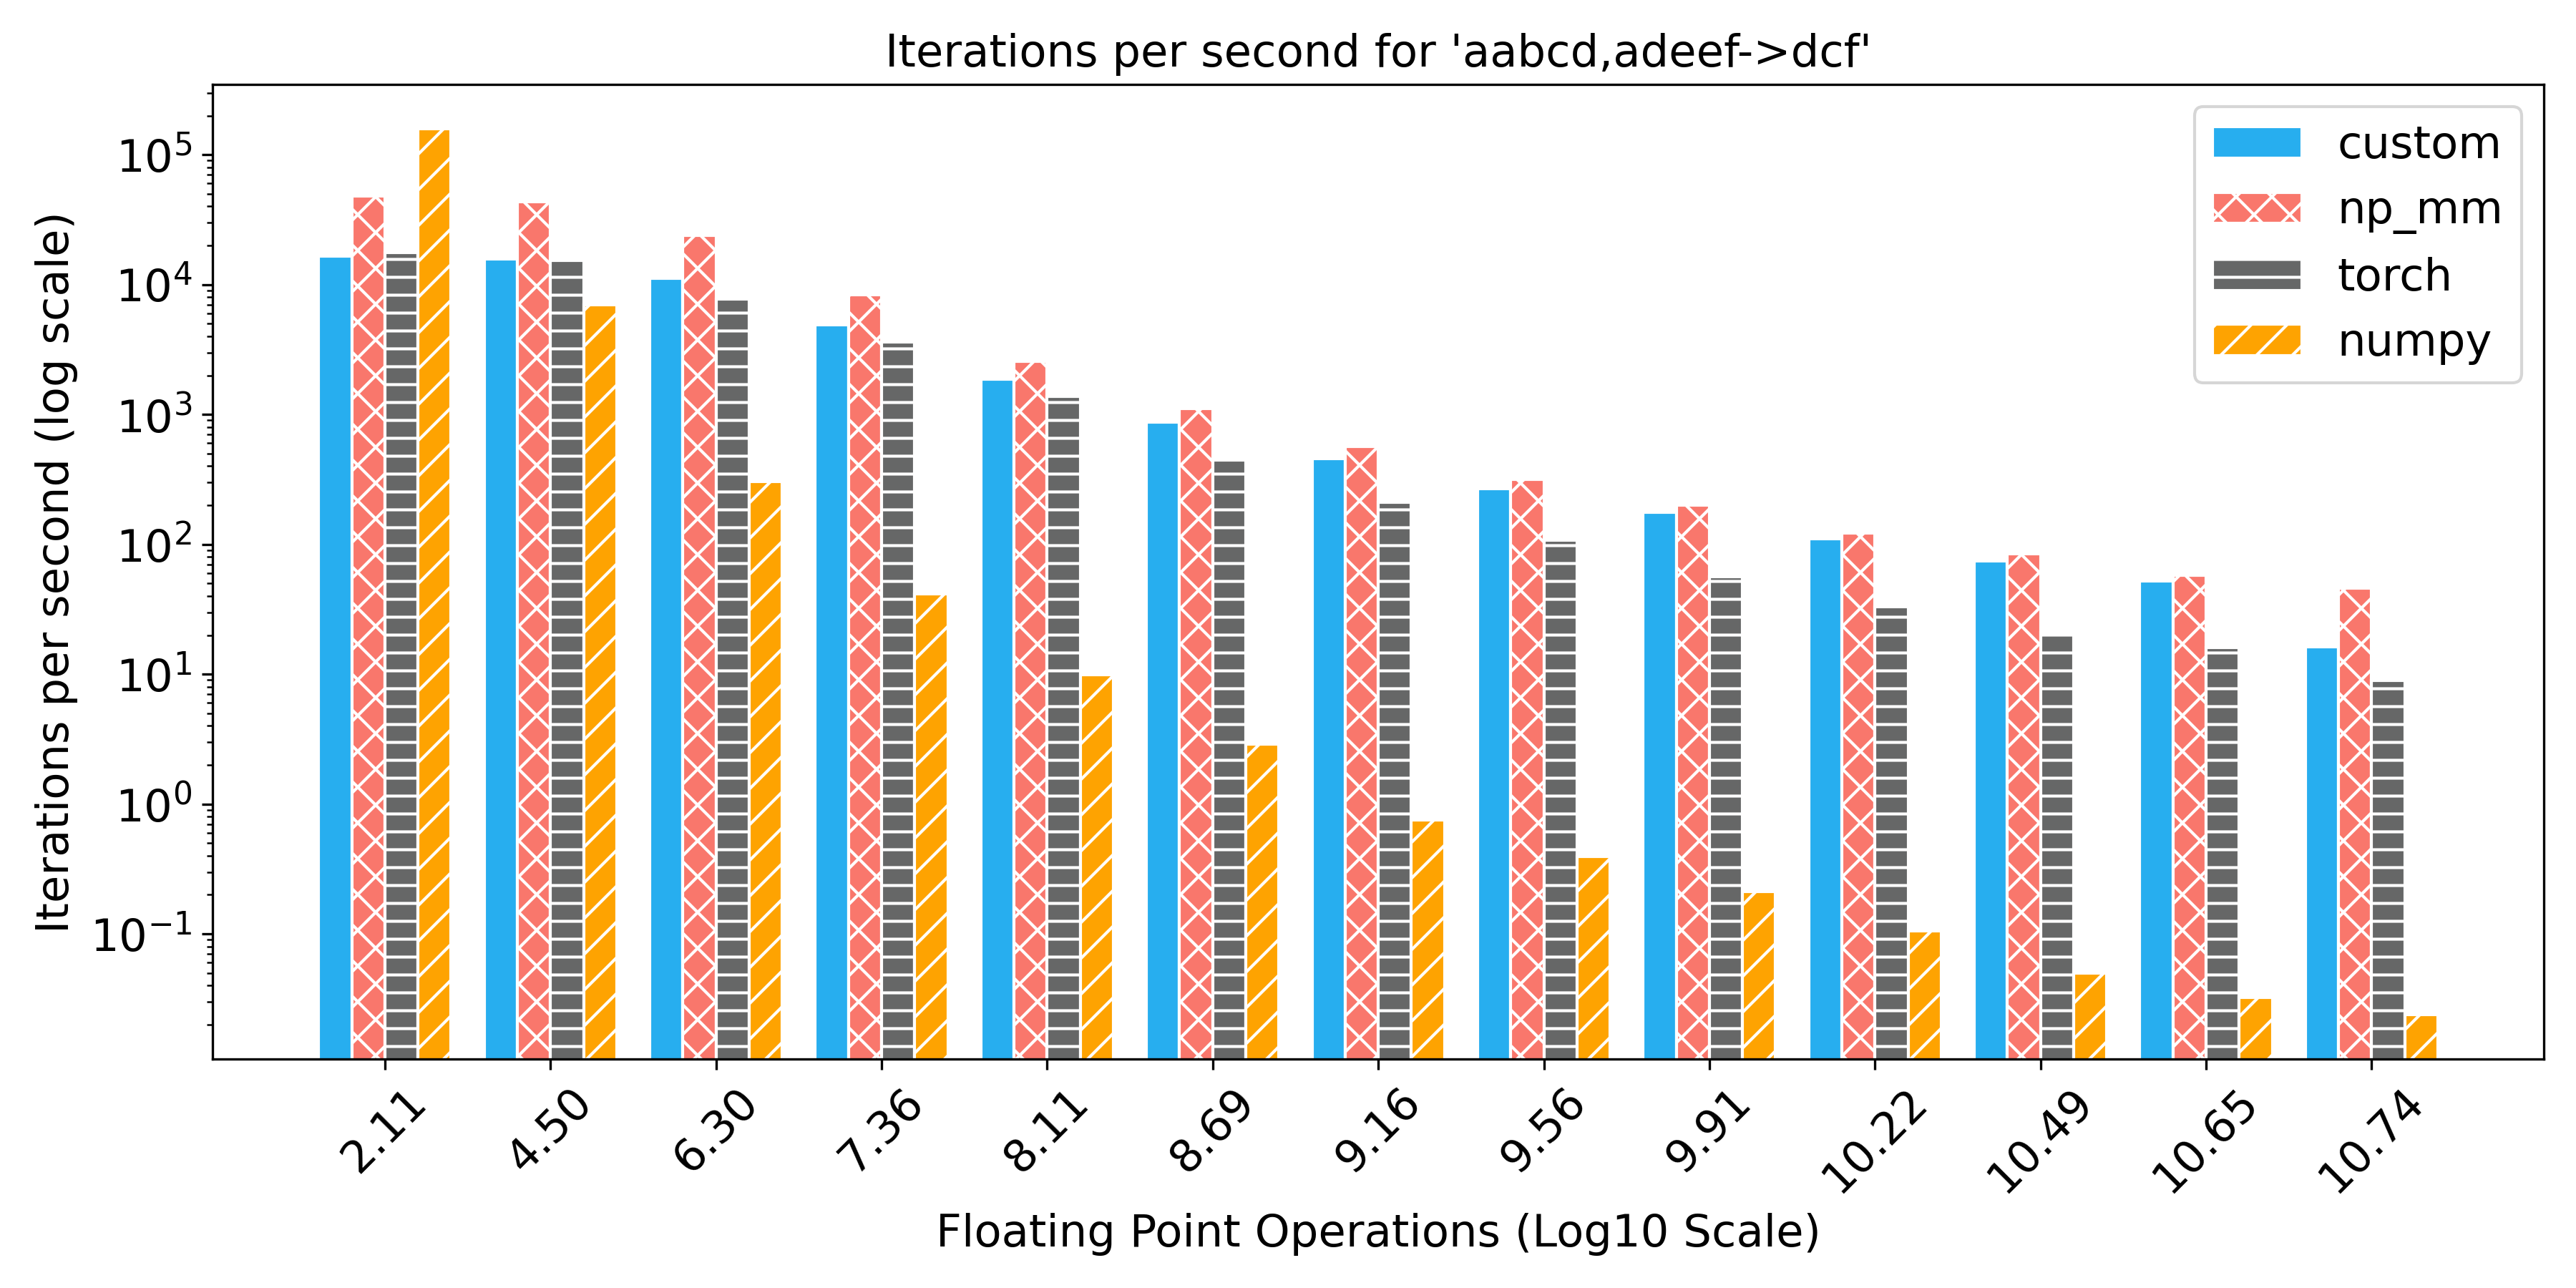
\includegraphics[width=0.49\textwidth]{images/aabcd_adeef__dcf.png} 
    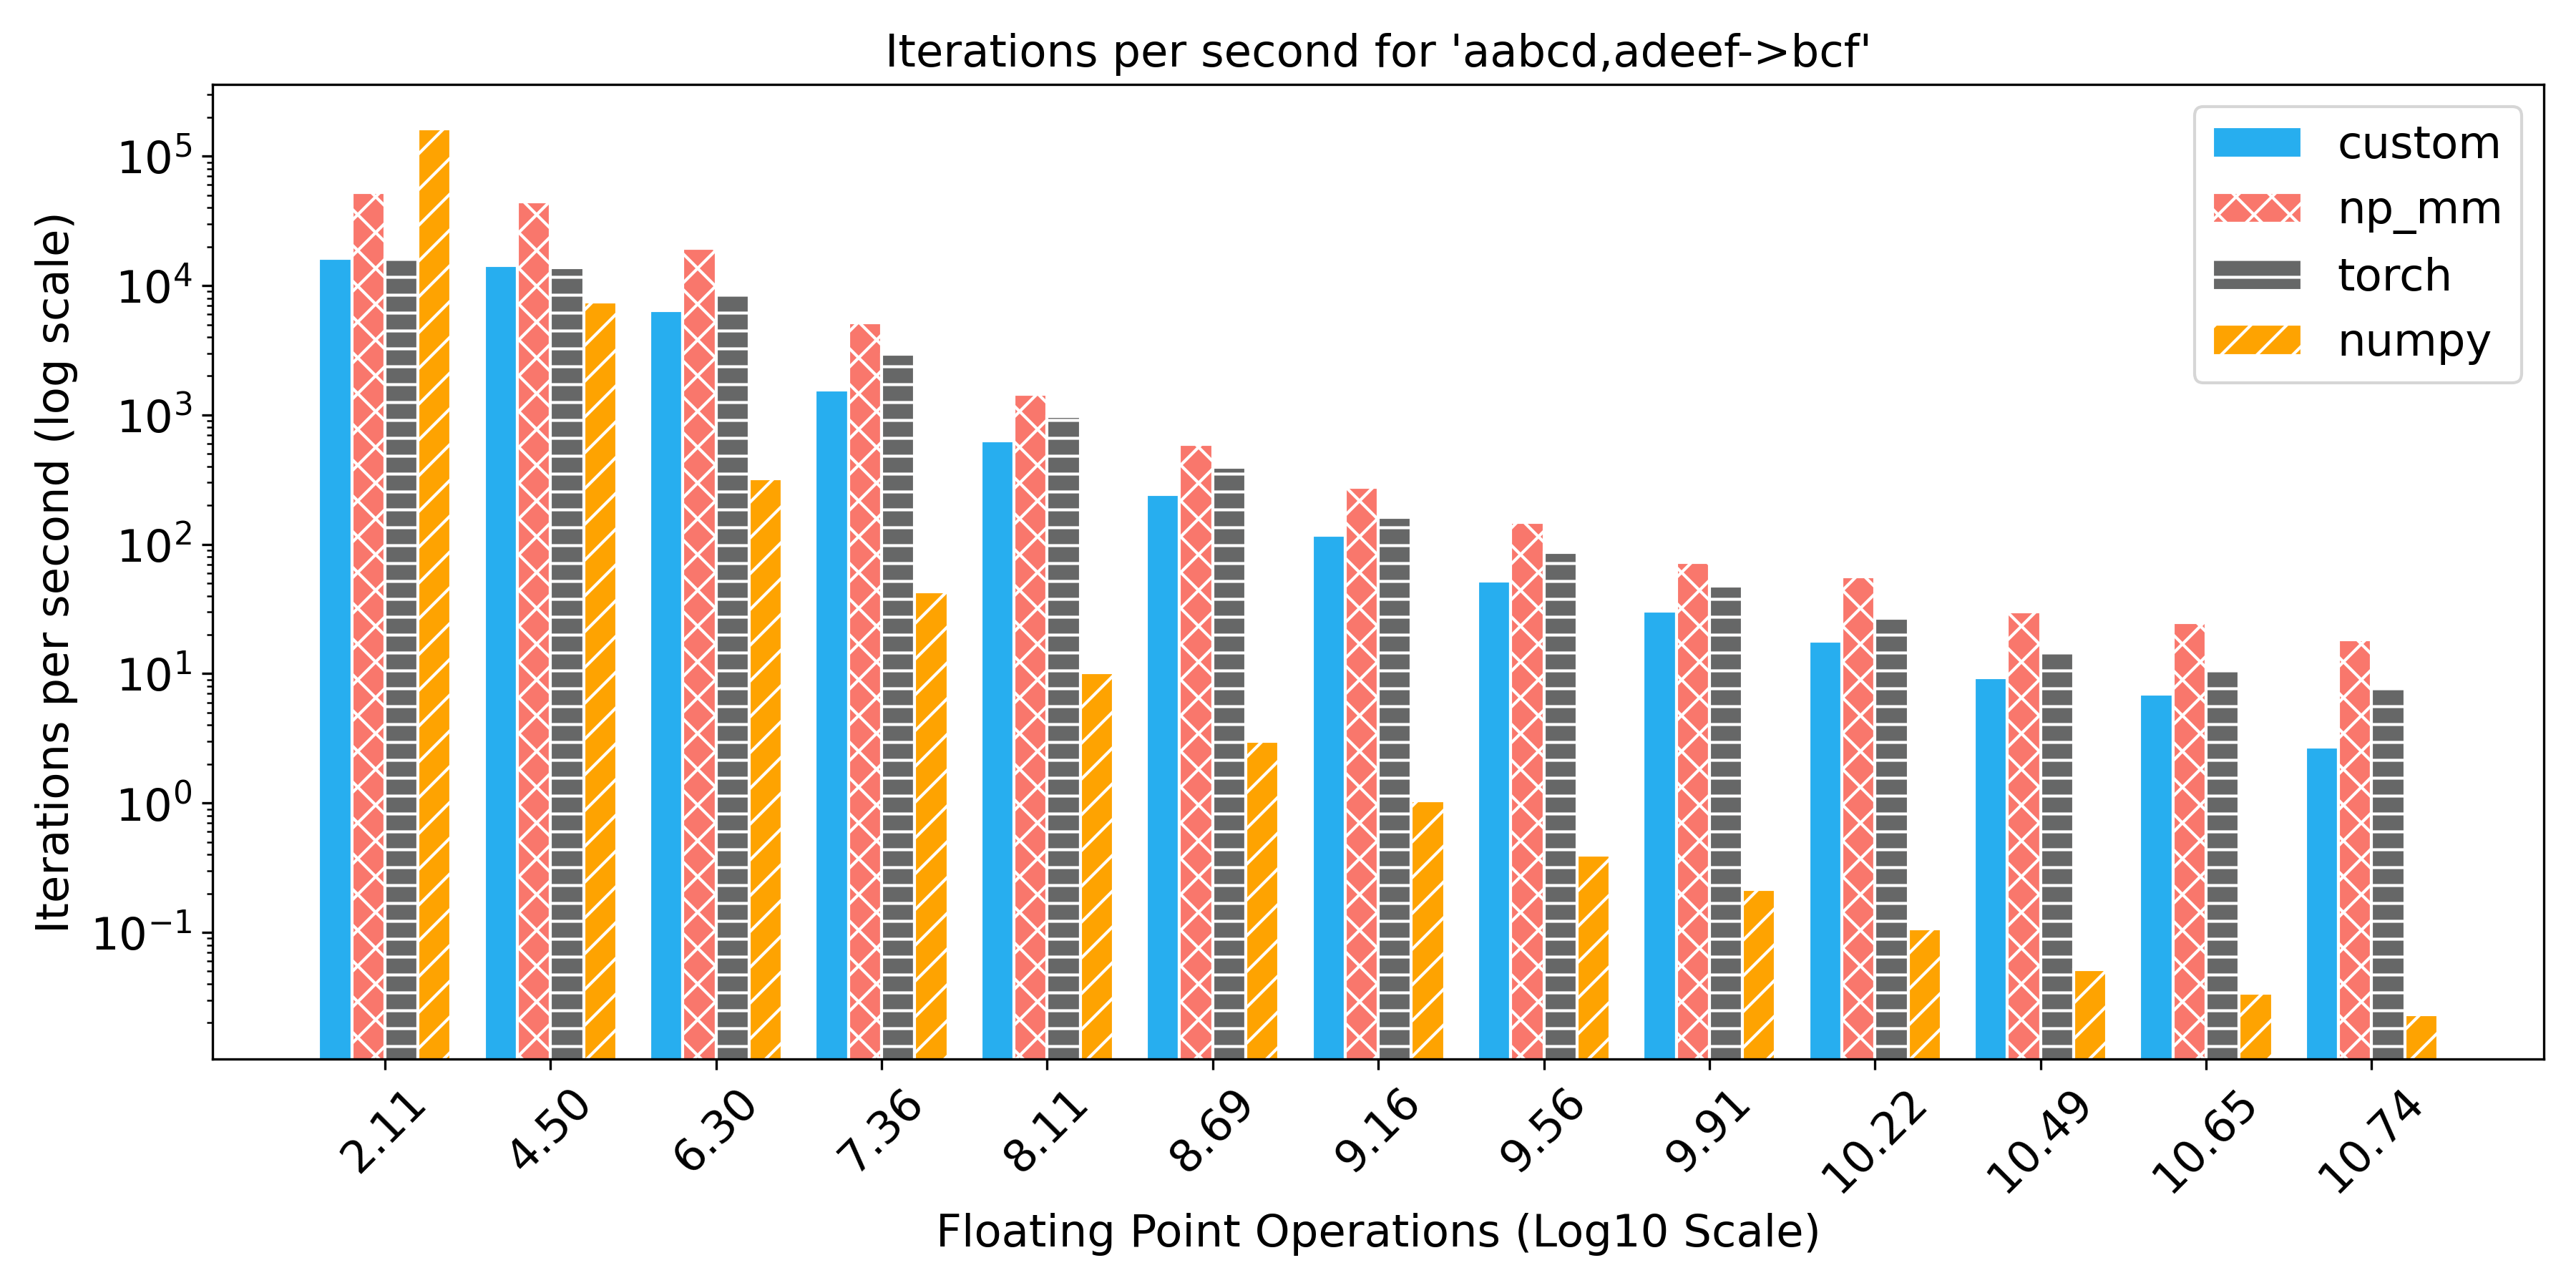
\includegraphics[width=0.49\textwidth]{images/aabcd_adeef__bcf.png} \\
    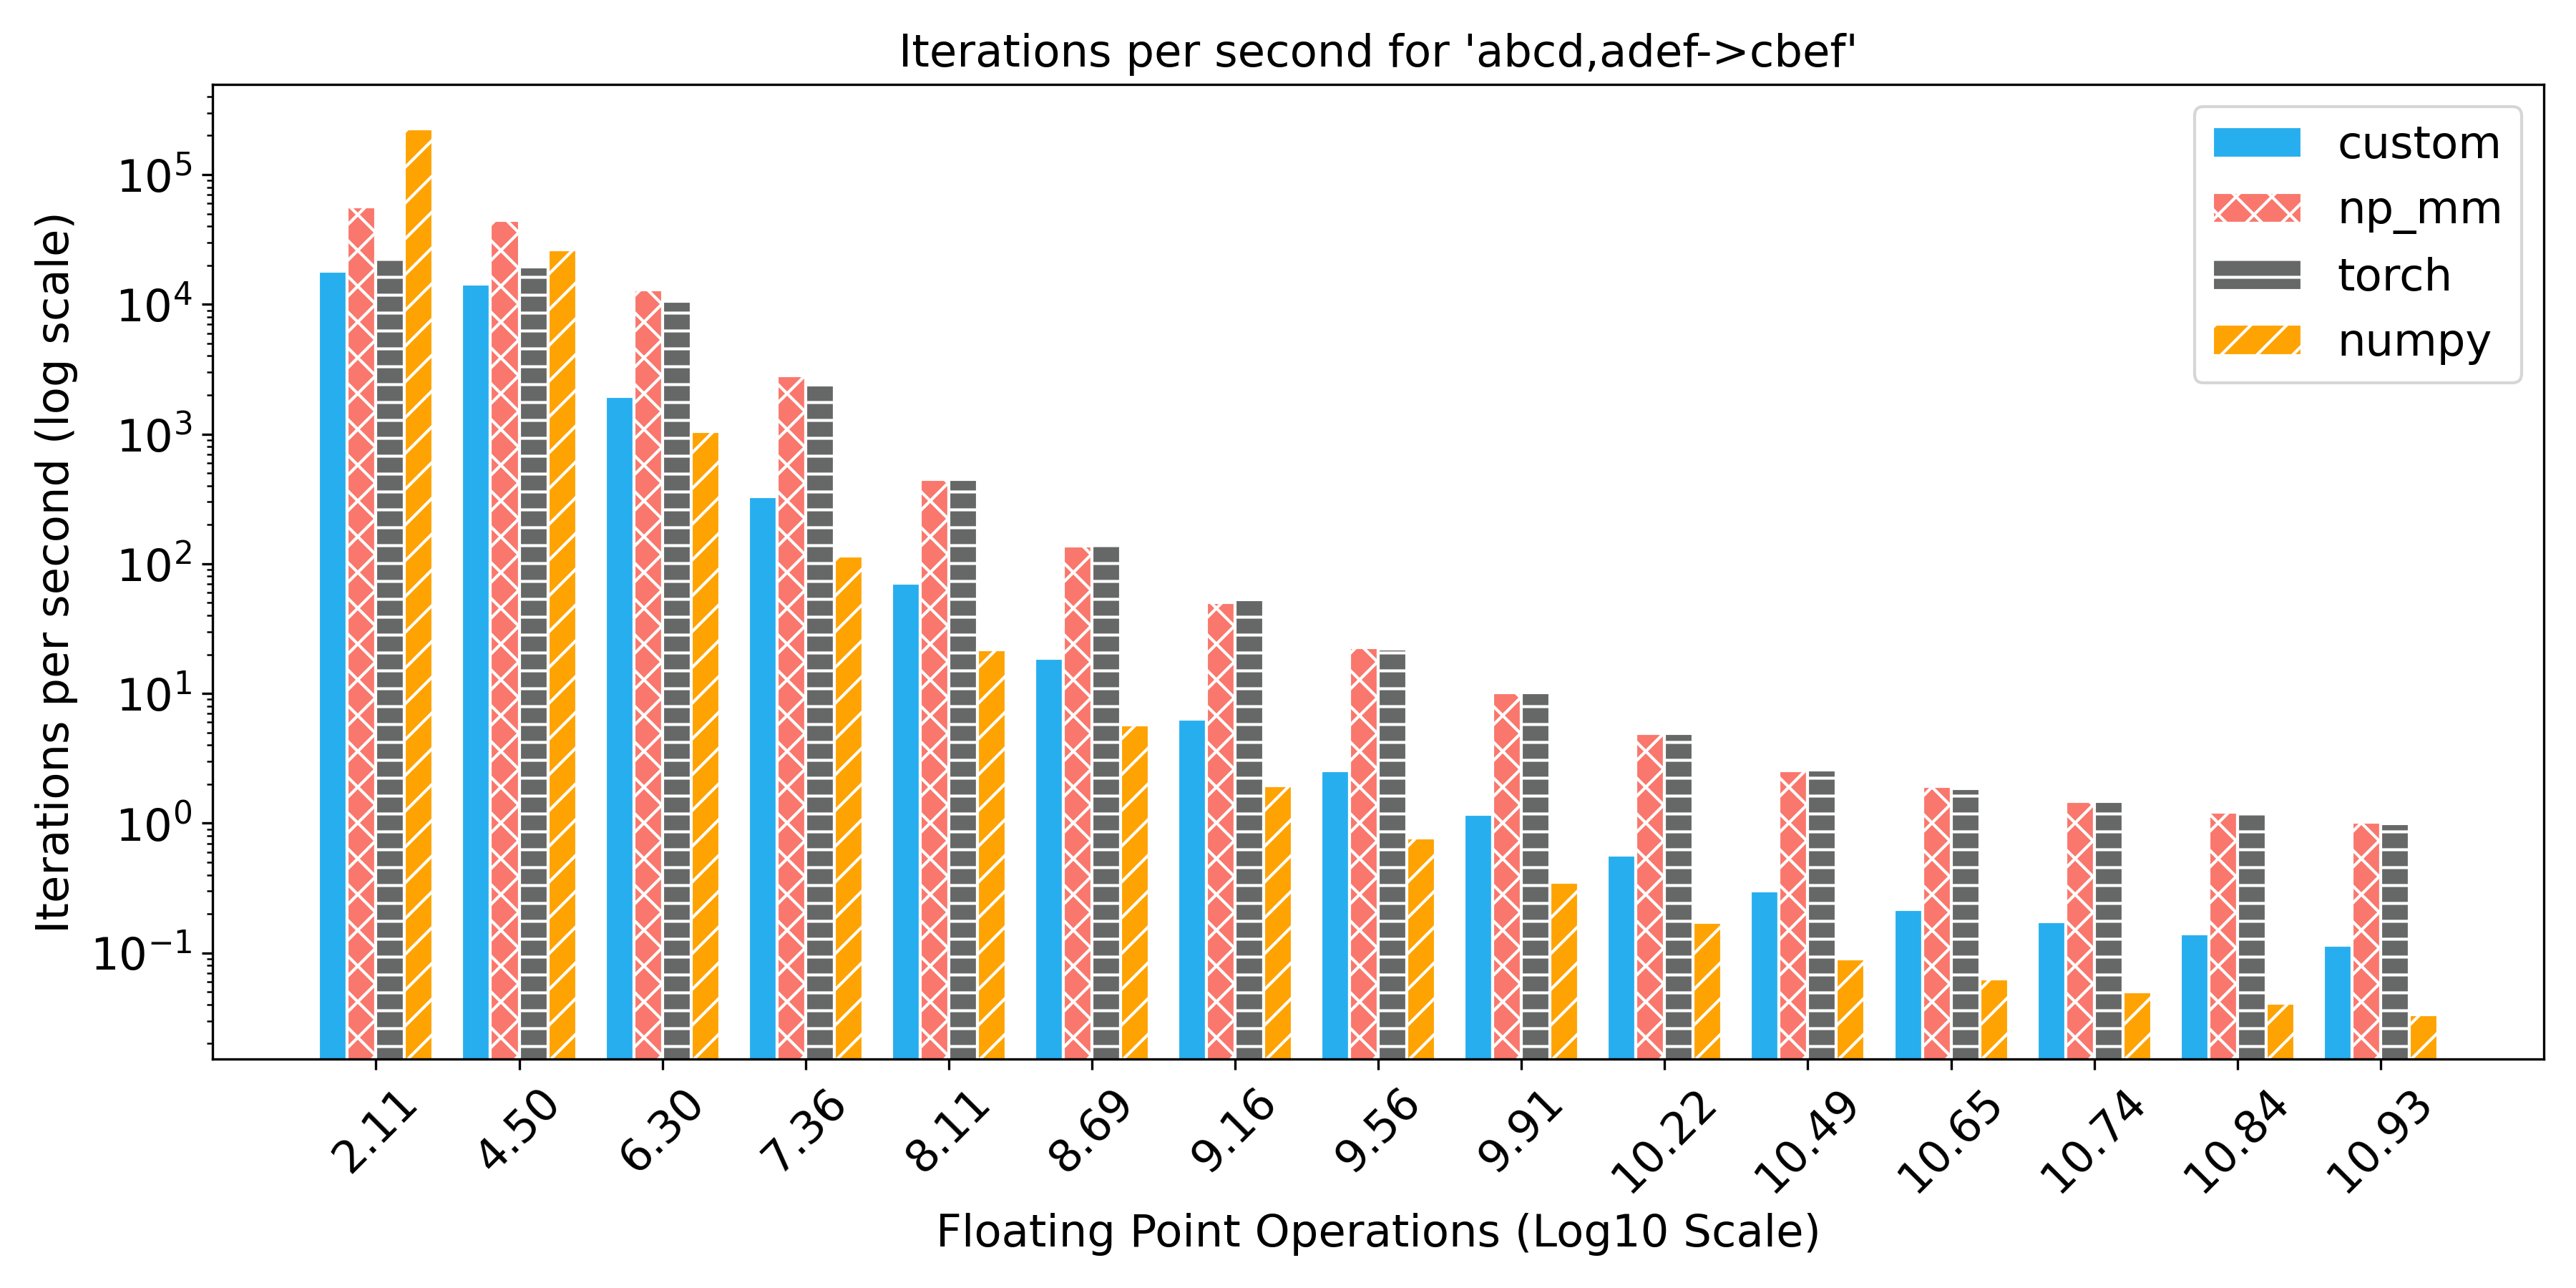
\includegraphics[width=0.49\textwidth]{images/abcd_adef__cbef.png}
    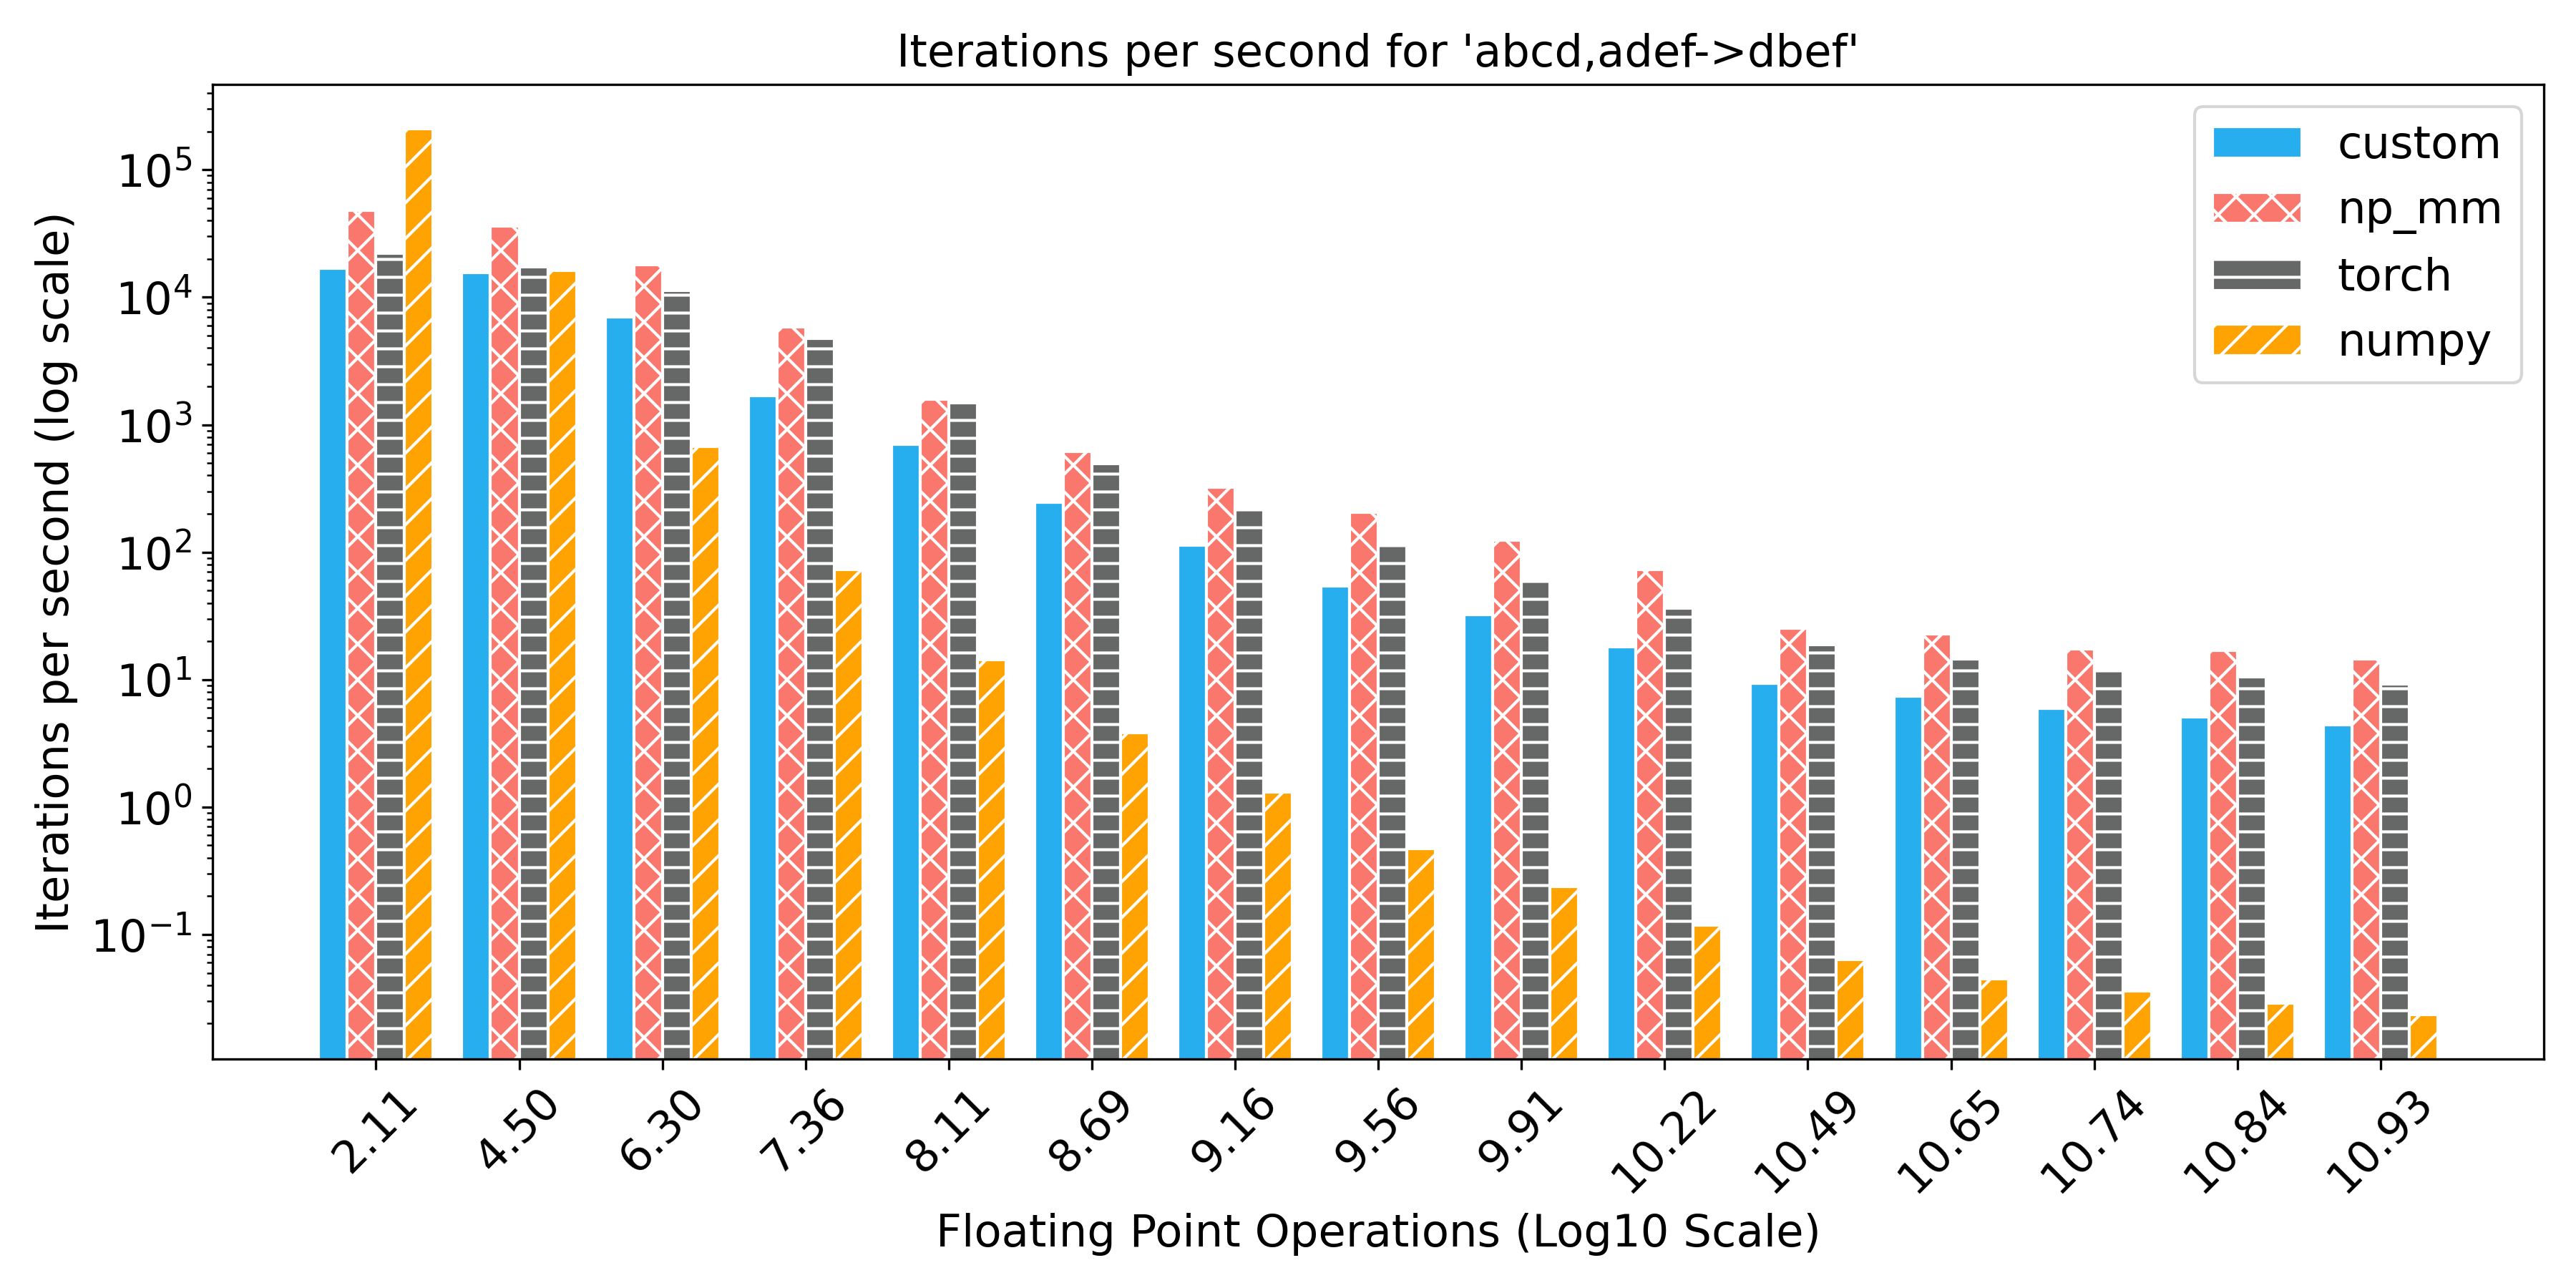
\includegraphics[width=0.49\textwidth]{images/abcd_adef__dbef.png}
    % Include your image
    \caption{Performance of the four backends over all four pairwise contractions. In all plots, the x-axis depicts the number of floating point operations corresponding to the gradually increased dimension sizes. }
\end{figure}
